\section{Resultados}
\label{cap2:resultados}
Ao ser executado, o script LUA realizou as seguintes ações:
\begin{itemize}
\item Reconstrução do circuito magnético no FEMM;
\item Definição do contorno;
\item Escolha dos materiais;
\item Definição do circuito elétrico;
\item Definição dos blocos (bobinas, material ferromagnético, ar);
\item Execução da função MESH (construção da malha de pontos);
\item Definição da linha de referência.
\item Construção do gráfico de densidade de fluxo magnético;
\item Construção do gráfico do potencial elétrico;
\item Construção do gráfico da da intensidade de campo;
\end{itemize}

\begin{figure}[H]
\centering
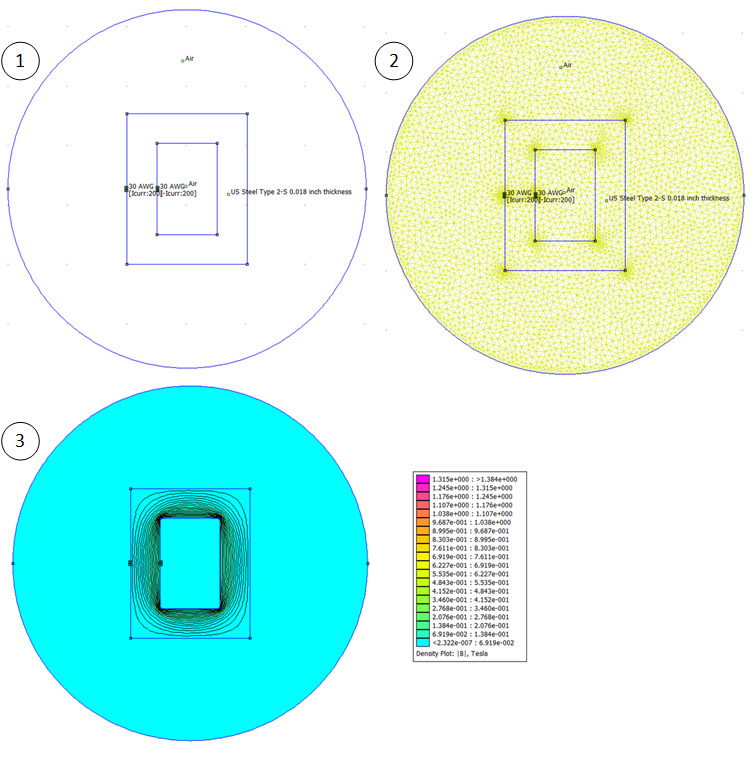
\includegraphics[scale=0.7]{img/assig2/results_1.png}
\caption[Resultados]{Resultados: (1) Representação do circuito magnético; (2) Malha de pontos gerada pelo FEMM; (3) Densidade de fluxo (Mapa de calor)}
\label{lua_mesh}
\end{figure}

\begin{figure}[H]
\centering
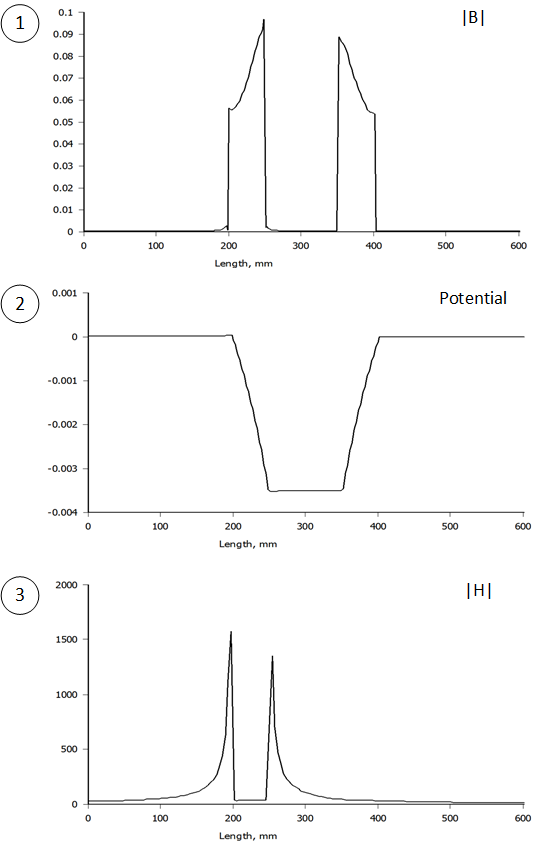
\includegraphics[scale=0.7]{img/assig2/results_2.png}
\caption[Gráficos]{Gráficos: (1) Densidade de fluxo magnético; (2) Potencial; (3) Intensidade de campo}
\label{lua_mesh}
\end{figure}


%\subsection{Análise do fluxo magnético, potencial e da intensidade de campo a partir de uma linha reta que passa pelo eixo central do circuito magnético}
%Para realizar a análise do fluxo magnético, potencial e da intensidade de campo, foi inserida no circuito magnético uma linha reta que coincide com o eixo central do mesmo, conforme ilustrado na figura \ref{loc_med}. Os gráficos das figuras \ref{graf_dfm}, \ref{graf_pot} e \ref{graf_ic} apresentam, respectivamente, a densidade de fluxo magnético (B), o potencial e a intensidade de corrente (H).
